
\chapter{Trace Evaluation}\label{ch:traceEvaluation}

The framework of testing is shown in Fig \ref{Proceduree}.
The work of testing devided into trace collection and trace evaluation.
At last chapter, we construct a tool to generate the traces of the websites automatically.
We use the tool SpecElicitor to help us making traces of Mobile Applications with the labels.
Even though we can easily generate lots of traces ,
it is still a heavy works to evaluate all traces.
Because the traces may lead to different result by some slight difference,
it needs people to check the traces case by case.
We develop a method to teach computer how to learn predicting a trace.

\begin{figure}[ht]
	\graphicspath{{pic/}}
	\begin{center}
		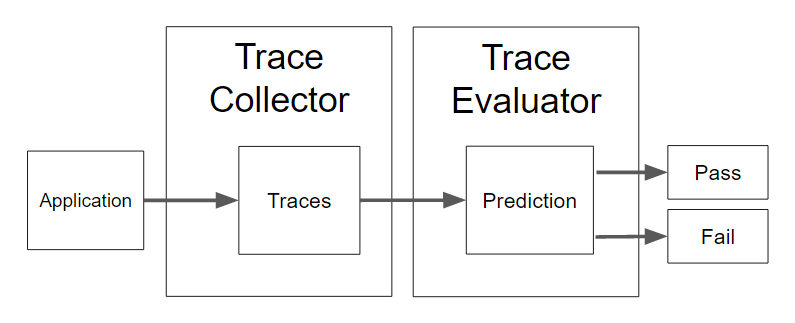
\includegraphics[width=0.8\textwidth]{Procedure.png}
	\end{center}
	\caption{ The framework of automated testing. }
	\label{Proceduree}
\end{figure}

%自動化產生traces後,evaluate仍需要大量人力
%為此設計一套能predict trace的framework

\clearpage

\section{Procedure}

The testing framework is shown in Fig[\ref{TraceEvaluation}].
An automated testing system can be devided into two parts,
one is automatically generating traces anf the another one is automated predicting the traces.
In the last chapter, we introduced a tool for automatically testing dynamic web applications.
With the tool WebTraceCollector and the tool SpecElicitor introduced in chapter 3,
we can collect web traces and android traces automaitcally.

In order to automated evaluating traces,
we need to construct a test oracle.
The test oracle may distinguishe the correct and incorrect behaviors of the system under test.
The simple ways are checking the behaviors manually, inserting assertions and detecing crash, error or failure in traces.
In our work, we use the machine learning method to achive the goal of evaluating traces automatically.
The method of machine learning we used in this paper is Support Vector Machine,
which needs collecting training set and testing set to train the predictive model.
Because the SVM is a supervised machine learining algorithm,
we have to labeled all traces for training.

The system will repeat the process of collecting traces of certain applications
and labeled the traces for training SVM model
until the accuracy of prediction is well enough.
The problem we occured will be how many traces we should collect to train a predictive model and
how to select the traces as training set and testing set.

%利用SVM cluster datas的能力
%將traces分成train set 和test set
%train set 先把trace的結果(pass/fail) label好
%然後用SVM train出一個model
%當收集越多的traces,train出來的model就會越準
%接著就可以用model來自動化evaluate traces

\begin{figure}[ht]
	\graphicspath{{pic/}}
	\begin{center}
		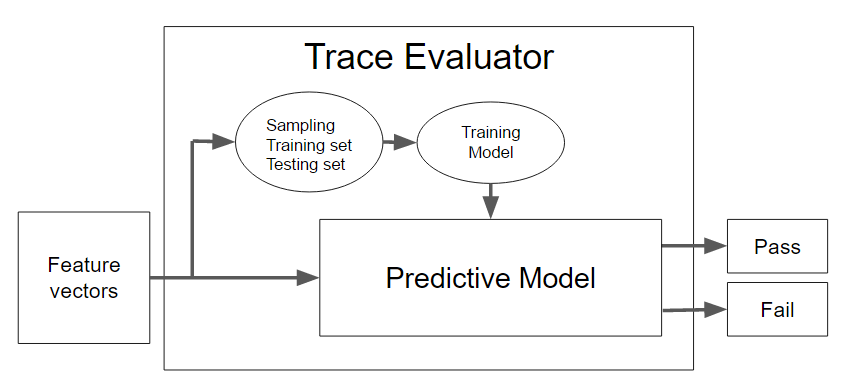
\includegraphics[width=0.8\textwidth]{TraceEvaluation.png}
	\end{center}
	\caption{ The framework of testing. }
	\label{TraceEvaluation}
\end{figure}

\clearpage

\section{Feature vector}

We hope that the method can not only predict the traces of one applications 
but also works on the traces between different application, even on the different platform,
so we need a specified defination of features that can work on different type of traces.

The tool SpecElicitor built a common sense model for labeling screens and actions during the test.
According to the common sense model, 
SpecElicitor can merge automata generated by different applications into one automata consist of label.
We select the normalized terms user labeled during the testing.
By generalizing the traces of similar applications, we construct a keyword dictionary.
The keyword dictionary is independently built on the database,
so we can easily updating the keywords.
The more traces we collect from several similar applications,
the more normalized keywords and it's synonyms we generalize.

We use the keyword dictionary as the specified feature used in trace evaluation.
In the case of the Android traces generated by SpecElicitor,
we directly get the feature of each states and edges.
By collecting those features, we convert the Android traces into a feature vector.
In the case of the traces generated by WebTraceCollector,
we need to extract the feature by string comparing between keywords and it's synonyms with the DOM tree of every state.

With the keyword dictionary, we can extract the features from the traces of web applications and mobile applications
and generate the feature vectors.
The vector is consist of integer numbers, which means the times the specific keyword appearing in the trace,
and the position of keywords in every vectors are stable.
A partial of feature vectors is shown in Fig \ref{featureVectors}.

We generalize the similar behaviors and represent the behaviors in normalized keywords between similar applications.
Therefore, the feature vectors extracted from traces of similar applications have same feature dimensions.
We can repeatedly use the keyword dictionary to automated extract features for reducing human effort.
After generating feature vectors, the SVM will training the model accroding the types of applications.
It is obvious that the keywords can seriously affect the training result.
If we can not precisely represent the incorrect behavior or failure in the traces by normalized keywords,
It will be hard to successfully extract the feature from traces.
However, the work of collecting keywords is a heavy work and can not be quickly complete.
We need constantly updating the keyword dictionary to increase the precision of keywords.

\begin{figure}[ht]
	\graphicspath{{pic/}}
	\begin{center}
		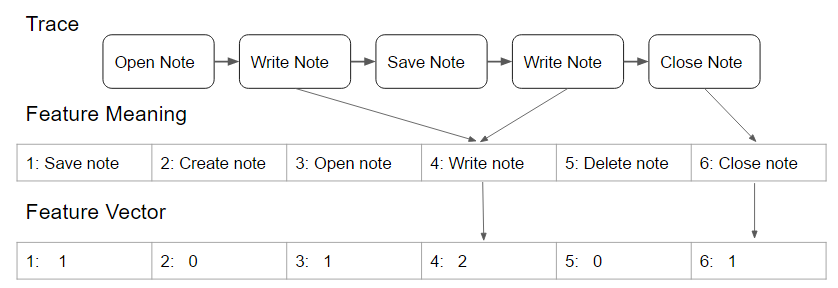
\includegraphics[width=0.8\textwidth]{vectors.png}
	\end{center}
	\caption{ Extracting the feature vectors. }
	\label{featureVectors}
\end{figure}

%為了要能將trace表現呈可運算的vector
%建立一個Common sense 的label 資料庫
%將APP和WEB的trace 轉換成label的 vector

\clearpage

\section{Sampling traces}

Before using the traces, we need to label it.
The precess of labeling traces as passed and failed is a hard work for human,
but it is necessary and can not be avoided in software testing.

How to select the traces to label into training set is another important problem.
If we can devide the traces precisely,
it can reduce the training work and the perfomance of predicting will be great.
However, it is too hard to find out which trace has the most informative feature.

In order to reduce human work,
The active learning algorithm can help us find out which traces should be labeled.
Active learning is a subfield of machine learning.
The studies about this field are gatherd by Settles\cite{ActiveLearning}
The active learning algorithm depends on the sampling strategy.
so we need a method to sample the trace more efficiently.
There are 3 sampling methods we could use, which are randomly sampling, greedy sampling and uncertainly sampling.
Randomly sampling just randomy pick a trace into training set.
Greedy sampling select the trace which can maximize the feature coverage.
Uncertainly sampling  select the trace whose prediction is the least confident.
We will implement them to find out which sampling method is the suitable to this system in the future.



